% Who is doing what:
% Jordan - 2.4.1 question 1, max-flow
% Darrin - RB tree
% Logan  - 2.1.1, 2.2.1
% Kate   - Example of max-flow

\documentclass[12pt]{amsart}

\usepackage[margin=0.75in]{geometry}

% Image setup
\usepackage{graphicx}
\graphicspath{{./images/}}

\title{}
\author{Jordan Dehmel, Kate Eckhart, Logan Humbert, Darrin Miller}
\date{2023}

\begin{document}

\maketitle

\newpage
\section{Section 2 Theoretical Questions}

    \subsection{Prove that the height of a Red-Black tree with
    n nodes is guaranteed to be $O(log n)$ in the worst
    case scenario. Provide a rigorous mathematical proof.}
    
    In this proof, we will first prove that the height of a
    2-3-4 tree is limited by $O(log n)$. Then, we will prove
    that any valid red-black tree can be converted directly into
    a 2-3-4 tree. Finally, we will note that, so long as height
    is measured only in black links, tree height is maintained
    by this conversion.

    A 2-3-4 tree, by its nature, only grows by pushing the root
    "upwards". The only time at which the height of such a tree
    increases is when a 4-node at the root splits, sending a
    node upwards to become the new root. In this case, the
    height of the tree uniformly increases by one for all leaf
    nodes. This means that the height of the tree is precisely
    equal for all leaf nodes no matter what.

    Now we will examine the equivalency between red-black trees
    and 2-3-4 trees. We will show that each node in a 2-3-4 tree
    corresponds to exactly one black link in a red-black tree,
    and that the only additions needed are red links.

    First, we will consider a 2-node. This is a node with two
    output links. This is equivalent to the standard node in a
    binary tree- no modifications are needed to modify it into
    red-black tree form.

    Next, we will consider a 3-node. This is a node with three
    output links. The leftmost represents the subtree wherein
    all nodes are less than the lesser item in the node. The
    rightmost similarly represents the subtree wherein all nodes
    are larger than the greater item, and the middle represents
    the subtree containing nodes who fit neither of these trees.

\begin{center}
    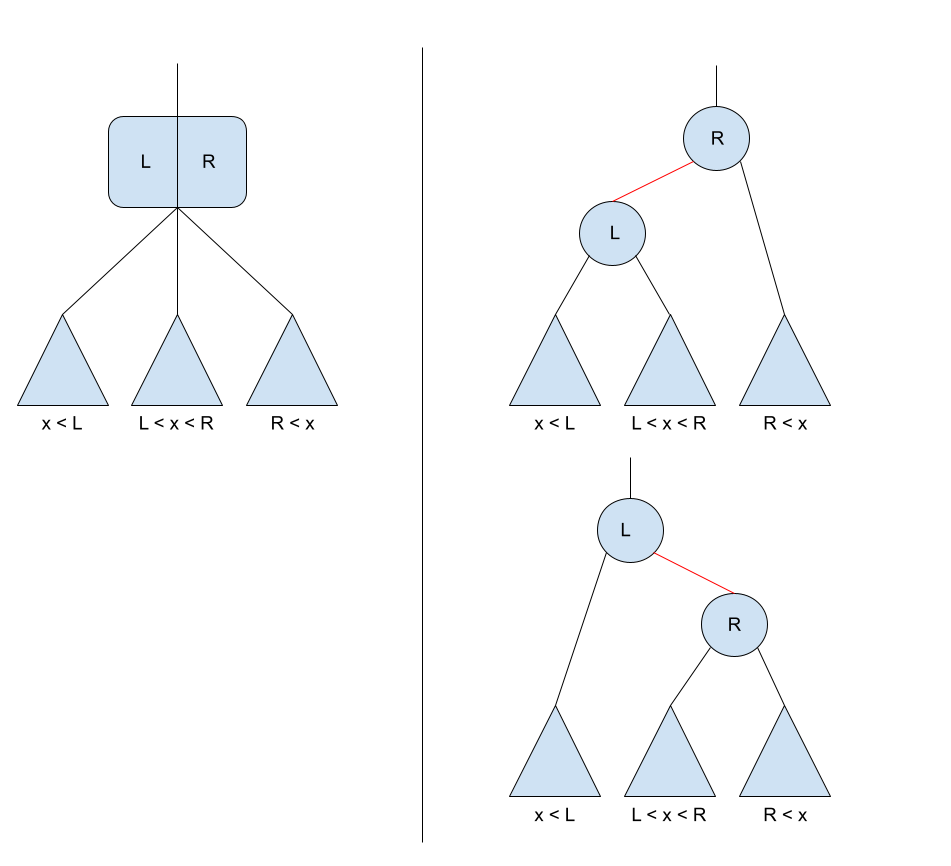
\includegraphics[width=0.65\textwidth]{rb_tree_1} \\
    A 3-node and its possible red-black tree versions. \\
    \vskip 1cm
\end{center}

    Since the height of a red-black tree is the number of black
    links the root must follow to get to a leaf, the two
    possible red-black subtrees above both have a height of $1$:
    the same height as the 2-3-4 tree they came from.

    The only remaining case is the 4-node. A 4-node usually only
    exists in a 2-3-4 tree for a moment before it is split
    apart. If we designate the $3$ items within the node as
    $a$, $b$, and $c$, then we say that (from left to right) the
    child links represent the ranges $x < a$, $a < x < b$,
    $b < x < c$, and $c < x$ for any item $x$ in the given
    child subtree. These cases, of course, can also be covered
    by an equivalent red-black tree, as shown below.

\begin{center}
    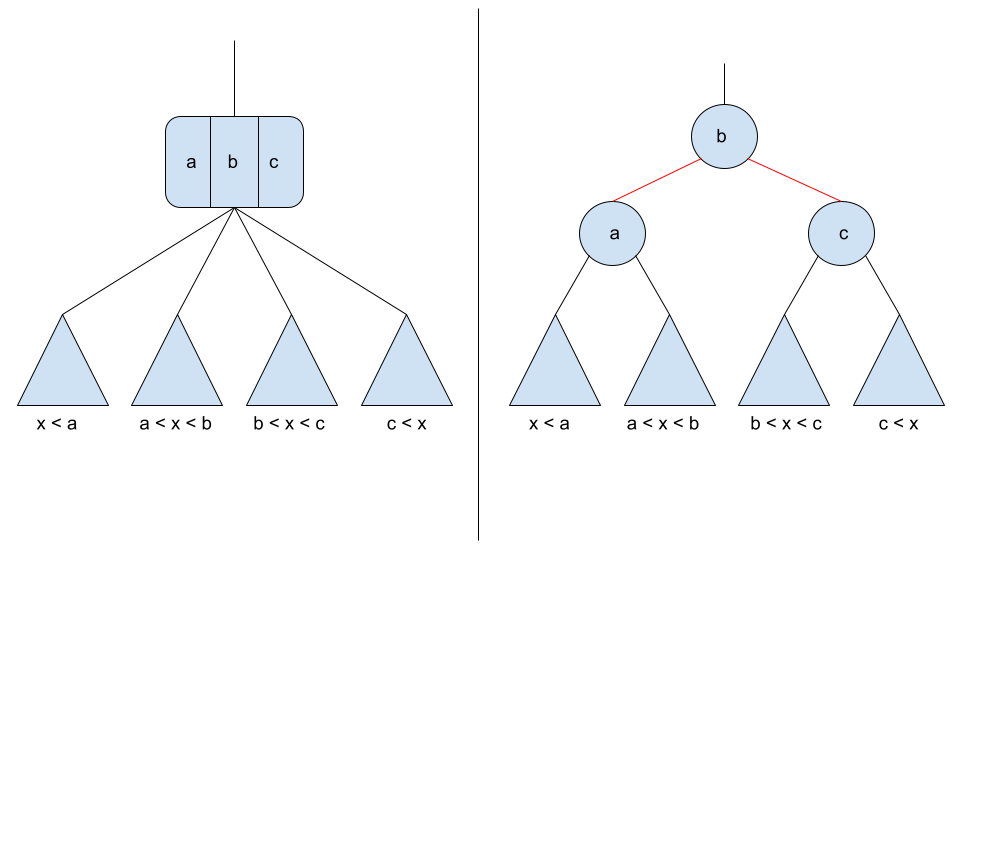
\includegraphics[width=0.65\textwidth]{rb_tree_2} \\
    A 4-node and its red-black tree version. \\
    \vskip 1cm
\end{center}

    Again, this red-black tree has the same height as its 2-3-4
    tree equivalent: $1$. Since we have accounted for all
    possible variations of red-black subtree herein, we can use
    the above rules to translate between red-black tree and
    2-3-4 tree. Therefore, any statement we make about 2-3-4
    trees holds for red-black trees.

    In the best-case scenario, a 2-3-4 tree (post 4-node
    splitting) will containing $n$ nodes will have a height of
    $log_3(n)$, where every node is a 3-node. At worst case, it
    will have a height of $log_2(n)$, where every node is a
    2-node. Since red-black and 2-3-4 trees are equivalent, we
    can thusly say that the worst-case height of a red-black
    tree of size $n$ is limited by $log_2(n)$ black links.

    \newpage
    \subsection{Discuss how Red-Black trees are used in modern
    databases and file systems to maintain balanced structures.
    Explain the trade-offs and advantages of using Red-Black
    trees in these contexts.}

\section{References}

    https://sedgewick.io/wp-content/themes/sedgewick/papers/2008LLRB.pdf

    https://www.cs.purdue.edu/homes/ayg/CS251/slides/chap13b.pdf

\end{document}